\documentclass{beamer}
\usetheme{CambridgeUS}
\usepackage{amsmath}
\usepackage{xcolor} % before tikz or tkz-euclide if necessary
\usepackage{tkz-euclide} % no need to load TikZ
\usepackage{multirow}

\usepackage[
backend=biber,
style=numeric,
sortlocale=de_DE,
natbib=true,
url=false, 
doi=true,
eprint=false
]{biblatex}

\definecolor{uamsred}{rgb}{0.6,0.2,0.2}
\setbeamercolor{mycolor}{fg=white,bg=uamsred}
\addbibresource{../../Bibliography/main_ML.bib}

\titlegraphic{\includegraphics[width=2cm]{../../Figures/UAMS_RGB.png}
}

\title{Statistical Machine Learning\\ Linear Discriminant and Performance Metrics}
\author{Horacio G\'omez-Acevedo\\ Department of Biomedical Informatics}
\begin{document}
	\begin{frame}[plain]
		\maketitle
	\end{frame}
	
	\begin{frame}{Linear Discrimination Motivation}
		We regularly use thresholds to label data points. 
		\begin{figure}
			\centering
			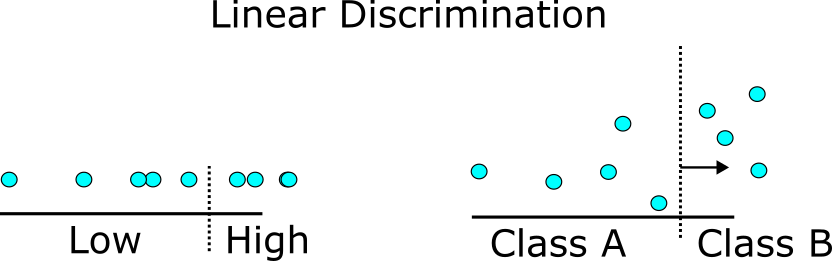
\includegraphics{../../Figures/fig_linear_disc.png}
		\end{figure}	
		Note that in the 2-dimensional case, we will be looking for a plane (or hyperplane in higher dimensions). One way to simplify finding for a plane is to identify a vector which is normal to the dividing plane. 
	\end{frame}
	
	\begin{frame}{Linear Discriminant Functions}
		A real-valued  function such as 
	
		\begin{equation}
			g(\mathbf{x})=\mathbf{w}^t \mathbf{x} +w_0	
			\label{eq:disc}
	\end{equation}	
	is called a {\bf discriminant function},
	where $\mathbf{w}$ is refer to as {\bf weight vector}, and  $w_0$  is normally called {\bf bias} (not the same as the statistical term). 
	
	For the discriminant function (\ref{eq:disc}) , we can define a two-category classifier (with classes $w_1$ and $w_2$) with the following rule:
	\begin{itemize}
		\item $\mathbf{x}\in w_1$ if $g(\mathbf{x}) >0$,
		\item $\mathbf{x}\in w_2$ if $g(\mathbf{x}) <0$
		\item if $g(\mathbf{x})=0$, then $\mathbf{x}$ can be assigned to either class.
	\end{itemize}
\end{frame}

\begin{frame}{Geometry related to the discriminant function}
	The equation $g(\mathbf{x})=0$ describes the {\bf decision surface} that separates both categories. If $\mathbf{x}_1$ and $\mathbf{x}_2$ are in the decision surface
	\begin{equation*}
		\mathbf{w}^t \mathbf{x}_1+w_0= \mathbf{w}^t \mathbf{x}_2+ w_0 \Rightarrow \mathbf{w}^t (\mathbf{x}_1 - \mathbf{x}_2)=0
	\end{equation*}
This implies that the vector $\mathbf{w}$ is normal to the hyperplane $H$ defined (generated) by the decision surface.
We can represent 
\begin{equation*}
	\mathbf{x}= \mathbf{x}_p+ r \frac{\mathbf{w}}{||\mathbf{w}||}
\end{equation*}
where $||\mathbf{w}||$ is the norm of $\mathbf{w}$ (i.e., $||\mathbf{w}||^2=\mathbf{w} \cdot \mathbf{w}$), $\mathbf{x}_p$ is the normal projection of $\mathbf{x}$ onto $H$ and $r$ is a signed distance (the sign depends on the side of the point $\mathbf{x}$ with respect to the separating plane $H$). More specifically,
\begin{equation*}
	r= \frac{g(\mathbf{x})}{||\mathbf{w}||}
\end{equation*}
\end{frame}

\begin{frame}{Discriminant Function }
	We can visualize these concepts with the following graph
\begin{figure}
	\centering
	\includegraphics[scale=0.05]{../../Figures/fig_duda_linear.jpg}
\end{figure}	
	
\end{frame}


\begin{frame}{Versatility of the Discriminant Functions}
	Whereas finding a point (plane or hyperplane) that splits the data into two categories, we can map our dataset to a higher dimension and find a solution.
	
	In the next figure, if we want to separate the interval in black from the intervals marked in red, it is clear that we cannot find a point from which the left will be on one class and right into another. But, if we use a discriminant function
	\begin{equation*}
		g(x)= a_0+ a_1 x + a_2 x^2
	\end{equation*}
	we can select a plane that splits those datasets.
	
\end{frame}

\begin{frame}{Discriminant functions (cont)}
	We can visualize this process with the following figure
	\begin{figure}
		\centering
		\includegraphics[scale=0.05]{../../Figures/fig_duda_non_convex_sep.jpg}
	\end{figure}
\end{frame}
\begin{frame}{Linearly separable case }
	Suppose we have a set of $n$ samples $\mathbf{y}_1,\ldots,\mathbf{y}_n$ and some of them are labeled $w_1$ and some labeled $w_2$. We want to determine the weights $\mathbf{a}$ in a linear discriminant function $g(\mathbf{x})=\mathbf{a}^t \mathbf{y}$
	
	First, we proceed with some sort of "normalization" which means that we replace all samples labeled $w_2$ by their negatives. Then the problem reduces to find a vector $\mathbf{a}$ such that 
	\begin{equation*}
		\mathbf{a}^t \mathbf y > 0
	\end{equation*}
for all of the samples. 

\begin{figure}
	\centering
	\includegraphics[scale=0.05]{../../Figures/fig_duda_positive_solution.jpg}
\end{figure}
\end{frame}

\begin{frame}{Gradient Descent Procedures}
		We need to find a solution to the set of linear inequalities $\mathbf{a}^t\mathbf{y}_i >0$. There may be several solutions, to determine the "best" solution is determined by the minimization of a criterion function $J(\mathbf{a})$.  The minimum (if exists) is called the "solution vector".

Recall that the gradient of a smooth function points towards the maximum for every point on the level surface. Thus, we need to use the negative of the gradient if we are to find the minimum.

\begin{figure}
	\centering
	\includegraphics[scale=0.35]{../../Figures/fig_gradient.png}
\end{figure}
\end{frame}

\begin{frame}{Gradient Descent Procedures (cont)}	
	The basic gradient descend goes as follows:
	
	\begin{enumerate}
		\item Chose an arbitrary weight vector $\mathbf{a}(1)$ 
		\item Compute $\nabla J (\mathbf{a})(1)$
		\item $\mathbf{a}(2)$ is obtained by moving the same distance from $\mathbf{a}(1)$ along the negative of the gradient.
	\end{enumerate}
We repeat this process following the formula
\begin{equation*}
	\mathbf{a}(k+1)= \mathbf{a}(k) -\eta(k) \nabla J (\mathbf{a}(k))
\end{equation*}
where $\eta >0 $ is called the {\bf learning rate } that sets the step size. We hope that the weight vectors will converge to a solution minimizing $J(\mathbf{a})$
\end{frame}


\begin{frame}{Confusion Matrix}
	A binary classifier placing instances in two classes $w_1$ and $w_2$ can make two types of error:
	\begin{itemize}
		\item it can assign an instance of $w_1$ into $w_2$
		\item it can assign an instance of $w_2$ into $w_1$
	\end{itemize}
The {\bf confusion matrix} allows us to summarize this information by putting it into a matrix in which each row represents the {\it actual} class, and each column represents the {\it predicted} class.

\begin{figure}
	\centering
	\includegraphics[scale=0.2]{../../Figures/fig_confusionmatrix.png}
\end{figure}

\end{frame}



\begin{frame}{Useful metrics}
	Once you have developed your binary classifier there are some common metrics to determine how well your classifier works.
	
	{\bf Precision} is defined as
	\begin{equation*}
		\textrm{precision}= \frac{TP}{TP+FP}
	\end{equation*}
	and the {\bf recall}  defined by the following expression
	\begin{equation*}
		\textrm{recall}= \frac{TP}{TP+FN}
	\end{equation*}
We also use another metric called the $F_1$ score that represents the harmonic mean of the precision and recall. 
\begin{equation*}
F_1= \frac{1}{\frac{1}{2}( \frac{1}{\textrm{precision}}+ \frac{1}{\textrm{recall}})}=\frac{TP}{TP+ \frac{FN+FP}{2}}
\end{equation*}
\end{frame}	

\begin{frame}{Observations about classifier metrics}
	\begin{itemize}
		\item False positives are  also known as {\it false alarm} or type I error.
		\item False negative are also known as {\it miss} or type II error.
		\item Recall is also referred to as {\it sensitivity} or {\it hit rate}.
		\item Precision is also called {\it positive predictive value}.
		\item In theory, you would like that precision and recall to be equal to 1. But this is not possible due to the {\bf precision-recall tradeoff}. 
	\end{itemize}


Suppose you are developing a new molecular technique (algorithm) to detect certain type of cancer  

{\bf Silly Scenario 1 }
You have tested your tool in vitro. You would like to detect as few false positives samples as possible, thus your precision must be very high while sacrificing recall.

{\bf Silly Scenario 2.}
If you proceed with human samples, 
a false positive can be financially costly due to the extra cost of further testing, but a false negative may cause harm to patients. Thus,  you would prefer higher recall sacrificing precision.
\end{frame}

\begin{frame}{Precision-Recall function}
	The so-called precision-recall function is obtained when we change the bias in our discriminant function and calculate the precision and recall. 
\begin{figure}
	\centering
	\includegraphics[scale=0.45]{../../Figures/precision_recall_vs_threshold_plot.png}
\end{figure}	
	
\end{frame}

\begin{frame}{ROC curve}
	The {\bf receiver operating characteristic curve (ROC)} plots the recall (true positive rate) against the {\it false positive rate}. 
	
	\begin{equation*}
		FPR= \frac{FP}{FP+TN}
	\end{equation*}
whereas the {\it true negative rate} or specificity 
\begin{equation*}
	TNR= \frac{TN}{FP+TN}
\end{equation*}
	Note that $FPR+TNR=1$, thus the ROC is a curve of the recall vs. 1-specificity, or FPR vs. TPR (if you want to keep everything positive!)
\end{frame}
\begin{frame}{ROC plot}
\begin{figure}
	\centering
	\includegraphics[scale=0.35]{../../Figures/roc_curve_plot.png}
\end{figure}
Normally, we calculate the "Area under the ROC curve" (AUROC) to compare our classification methods.

{\bf Note} If you have ROC curve close to the dotted line, your classifier is not doing better than a random choice.
\end{frame}
\begin{frame}{Multilabel and Multioutput Classification}
	In cases where you want to classify instances in multiple classes simultaneously, some classifiers (e.g., KNN) allow you to use that type of classification, and it is named (not surprisingly {\bf multilabel classification}. )
	
	Note that the confusion matrix can be extended to multiple classification, whereas some other metrics are for binary classification problems.
	
	On the other hand the {\bf multioutput classification} is similar to a multilabel but each of the labels can have more than two possible values (e.g., discrete output)
\end{frame}

\begin{frame}{What have we learned?}
	\begin{itemize}
		\item Linear discriminant functions and their use in classification.
		\item The definition of a confusion matrix.
		\item Precision and recall and their trade off. 
		\item Receiver operating characteristic curves (ROC)

		
	\end{itemize}
\end{frame}


\begin{frame}{References}
	

Materials and some of the pictures are from \citep{James2015}, \citep{duda}, and \citep{geron2}
\printbibliography 

	
	I have used some of the graphs by hacking TiKz code from StakExchange and other old tricks of \TeX
\end{frame}		

\end{document}